\textbf{Motivation.} Implementing the instant messenger system, we consider applying a well-known N-tier
Monolithic Architecture [\cite{bucchiarone2018monolithic}], which provides a time-proven model that allows software
developers to create flexible and reusable applications.

However, during the implementation of monolith it is very important to avoid the cases of crucial over-engineering
of the system that leads to useless complication of the code base.
For the developers, it is a vital point to follow the KISS [\cite{alwin2016kiss}] and YAGNI [\cite{da2018evolution}]
software development principles in order not to reach
\href{https://github.com/smartstore/SmartStoreNET/blob/4.x/src/Presentation/SmartStore.Web/Controllers/CatalogHelper.cs}
{thousands lines}
of code in a single class.

One would suggest to use nowadays popular Microservices Architecture, thinking about scalability [\cite{brataas2004exploring}],
an ability of the system to handle large numbers of users distributed over geographically large areas without
notably affecting the overall performance of the system.
However, the effect of Microservices is being felt only for quite large and complex systems,
not the case of our yet simple application.
According to \href{https://martinfowler.com/bliki/MonolithFirst.html}{Martin Fowler},
\begin{quote}
    \textit{you shouldn't start a new project with microservices, even if you're sure your application will be big enough to
    make it worthwhile.}
\end{quote}
which is so-called \textit{Monolith first} approach.
Makes sense to begin an implementation from \textit{Modular monolith}, a monolith with minimized coupling between the
software components, where splitting to microservice won't be a time and financial expensive operation.
Following plot demonstrates the relation between the complexity and profits between monolith and microservices

\begin{figure}[H]
    \centering
    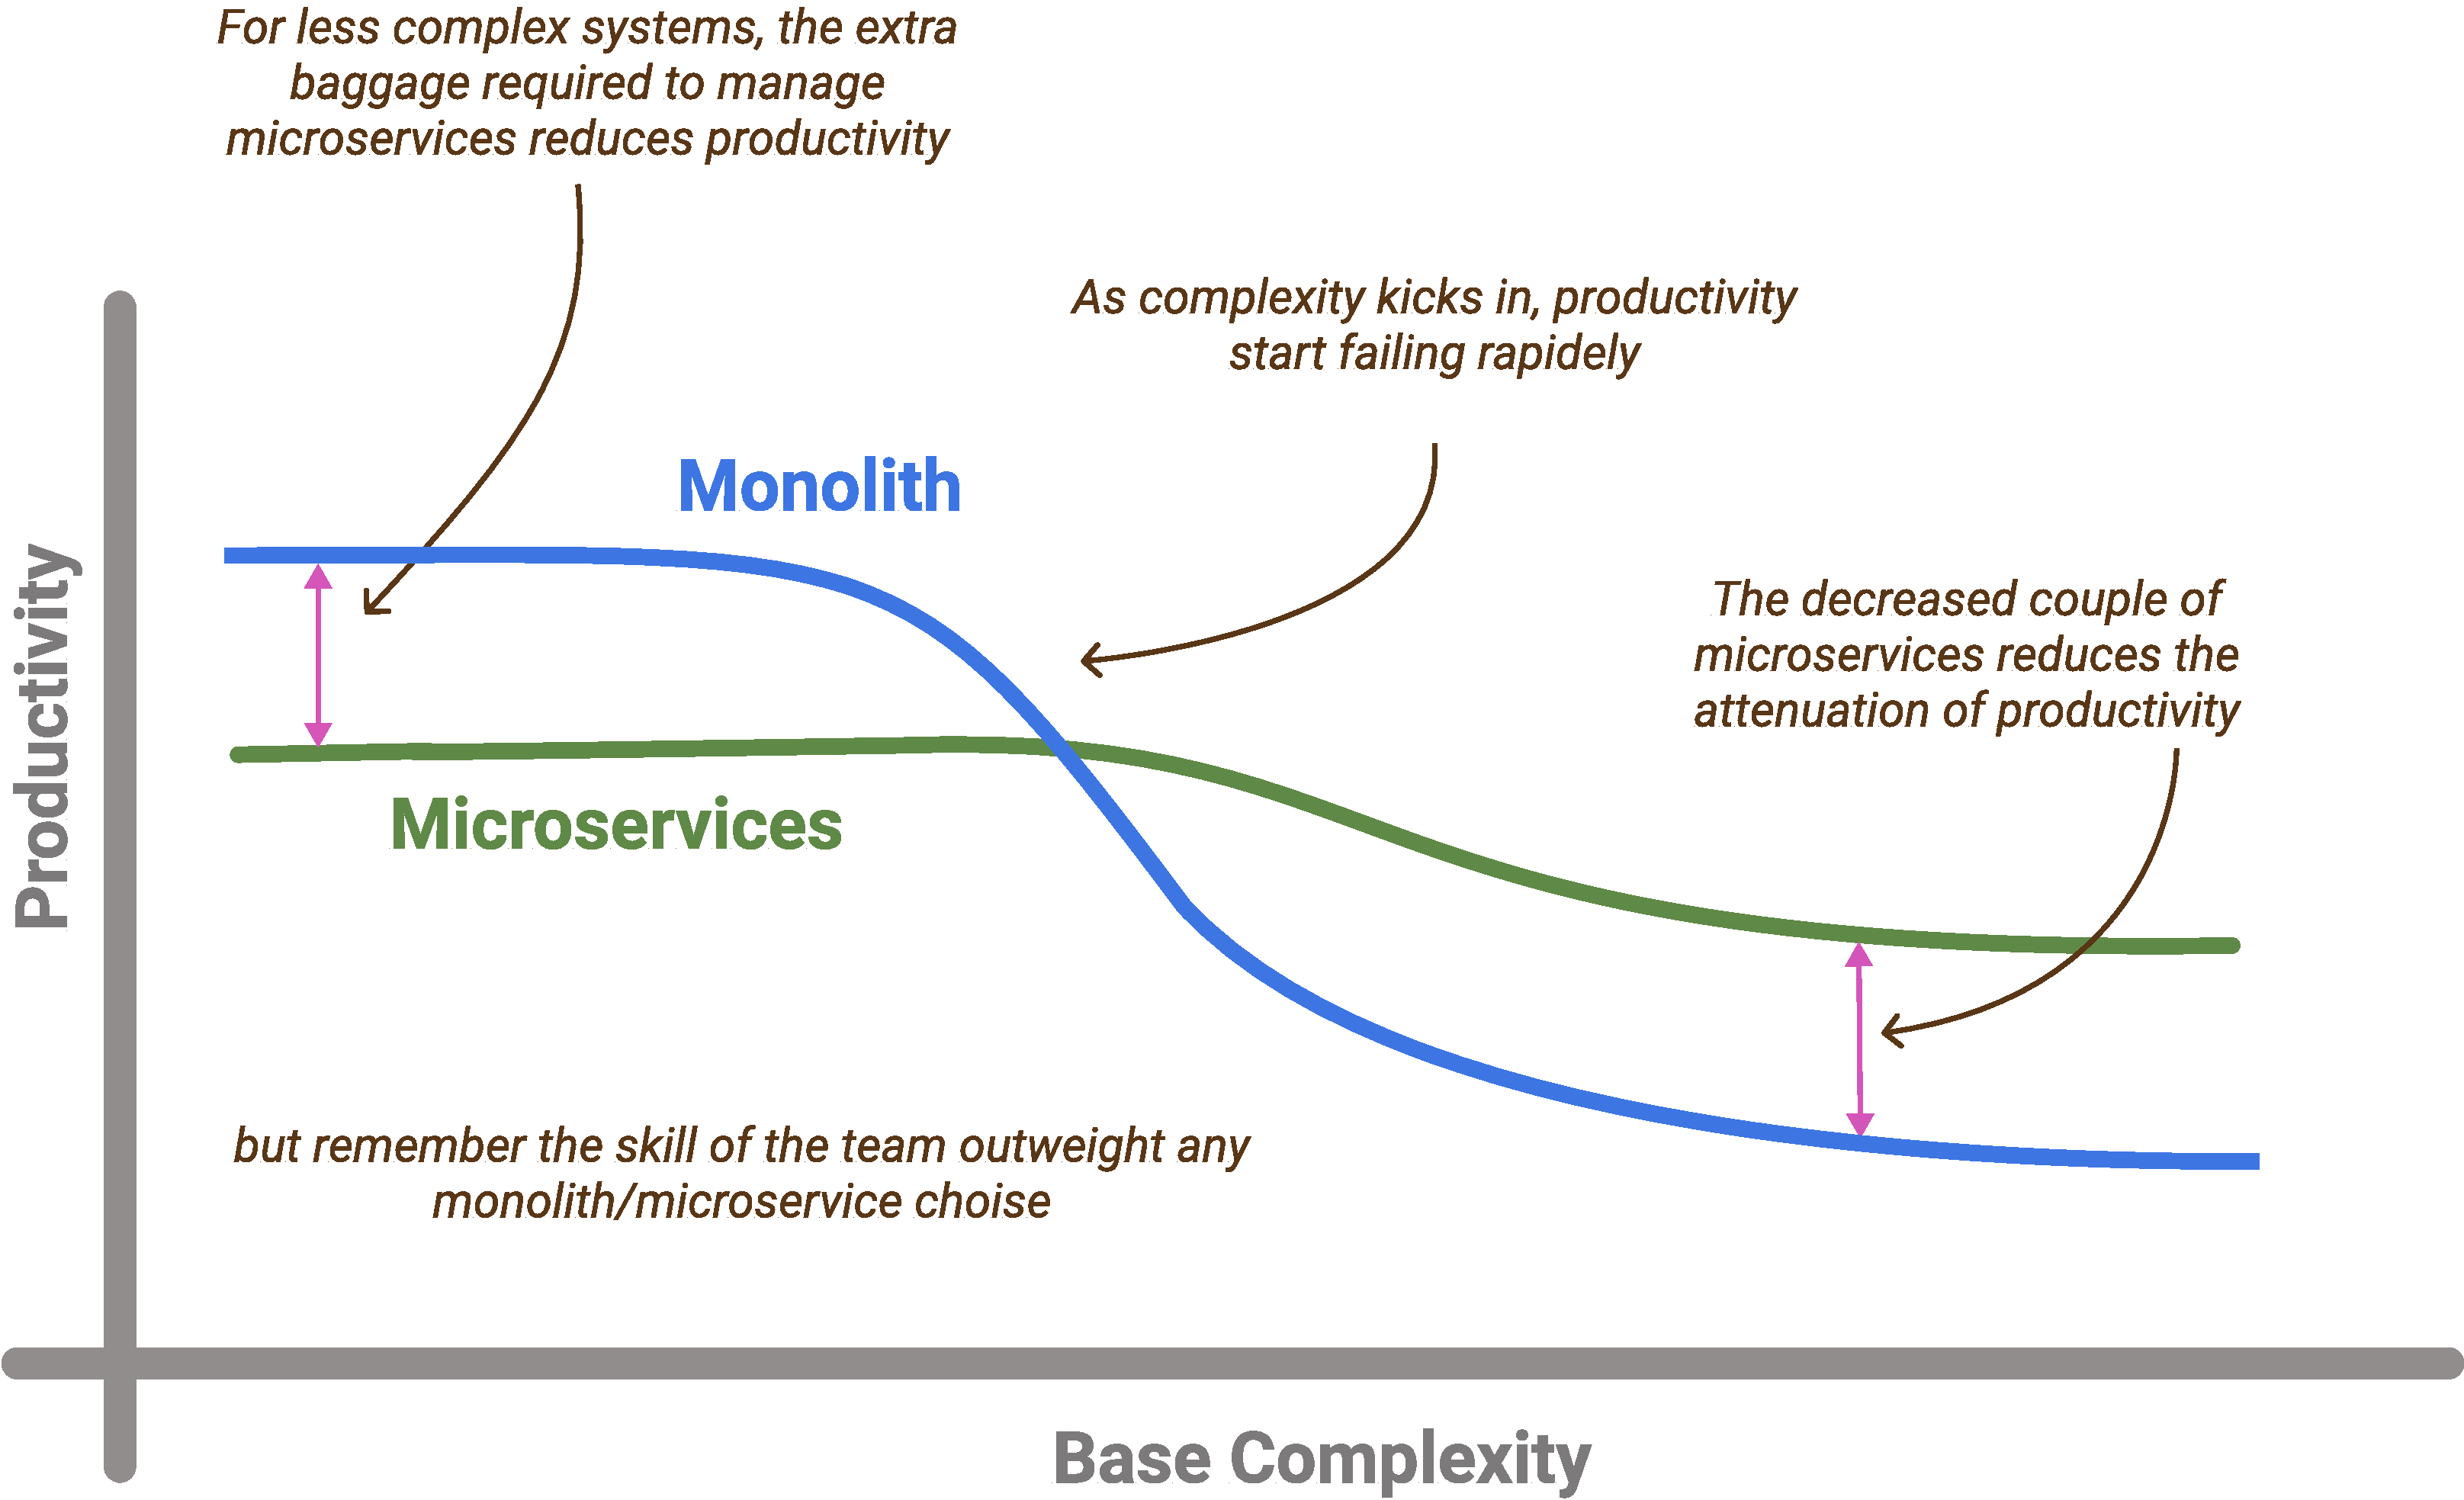
\includegraphics[width=1\textwidth]{Pictures/02_Monolith_and_Microservices_complexity}
    \caption{Relation between system complexity and architectures.
    Source: \href{https://martinfowler.com/bliki/MicroservicePremium.html}{Martin Fowler.}}
    \label{fig:monolith_vs_microservice}
\end{figure}

A layered architecture usually consists of Presentation layer, Business logic layer, Data access layer.
By segregating the project into layers, developers reach the options to modify or add a specific layer
without reworking the entire application.

\begin{itemize}
    \item \textit{Presentation Layer.} Graphic user interface or API gateway.
    \item \textit{Application Logic.} Encapsulates the means of interaction with user.
    For example, push-notifications e-mail notification, sms notifications etc.
    \item \textit{Business Logic.} Encapsulates the logic of clint's request handling.
    For example, service layer.
    \item \textit{Data Access Layer.} Responsible for logging, database access and other services required to support
    Business Logic layer.
\end{itemize}

\begin{figure}[H]
    \centering
    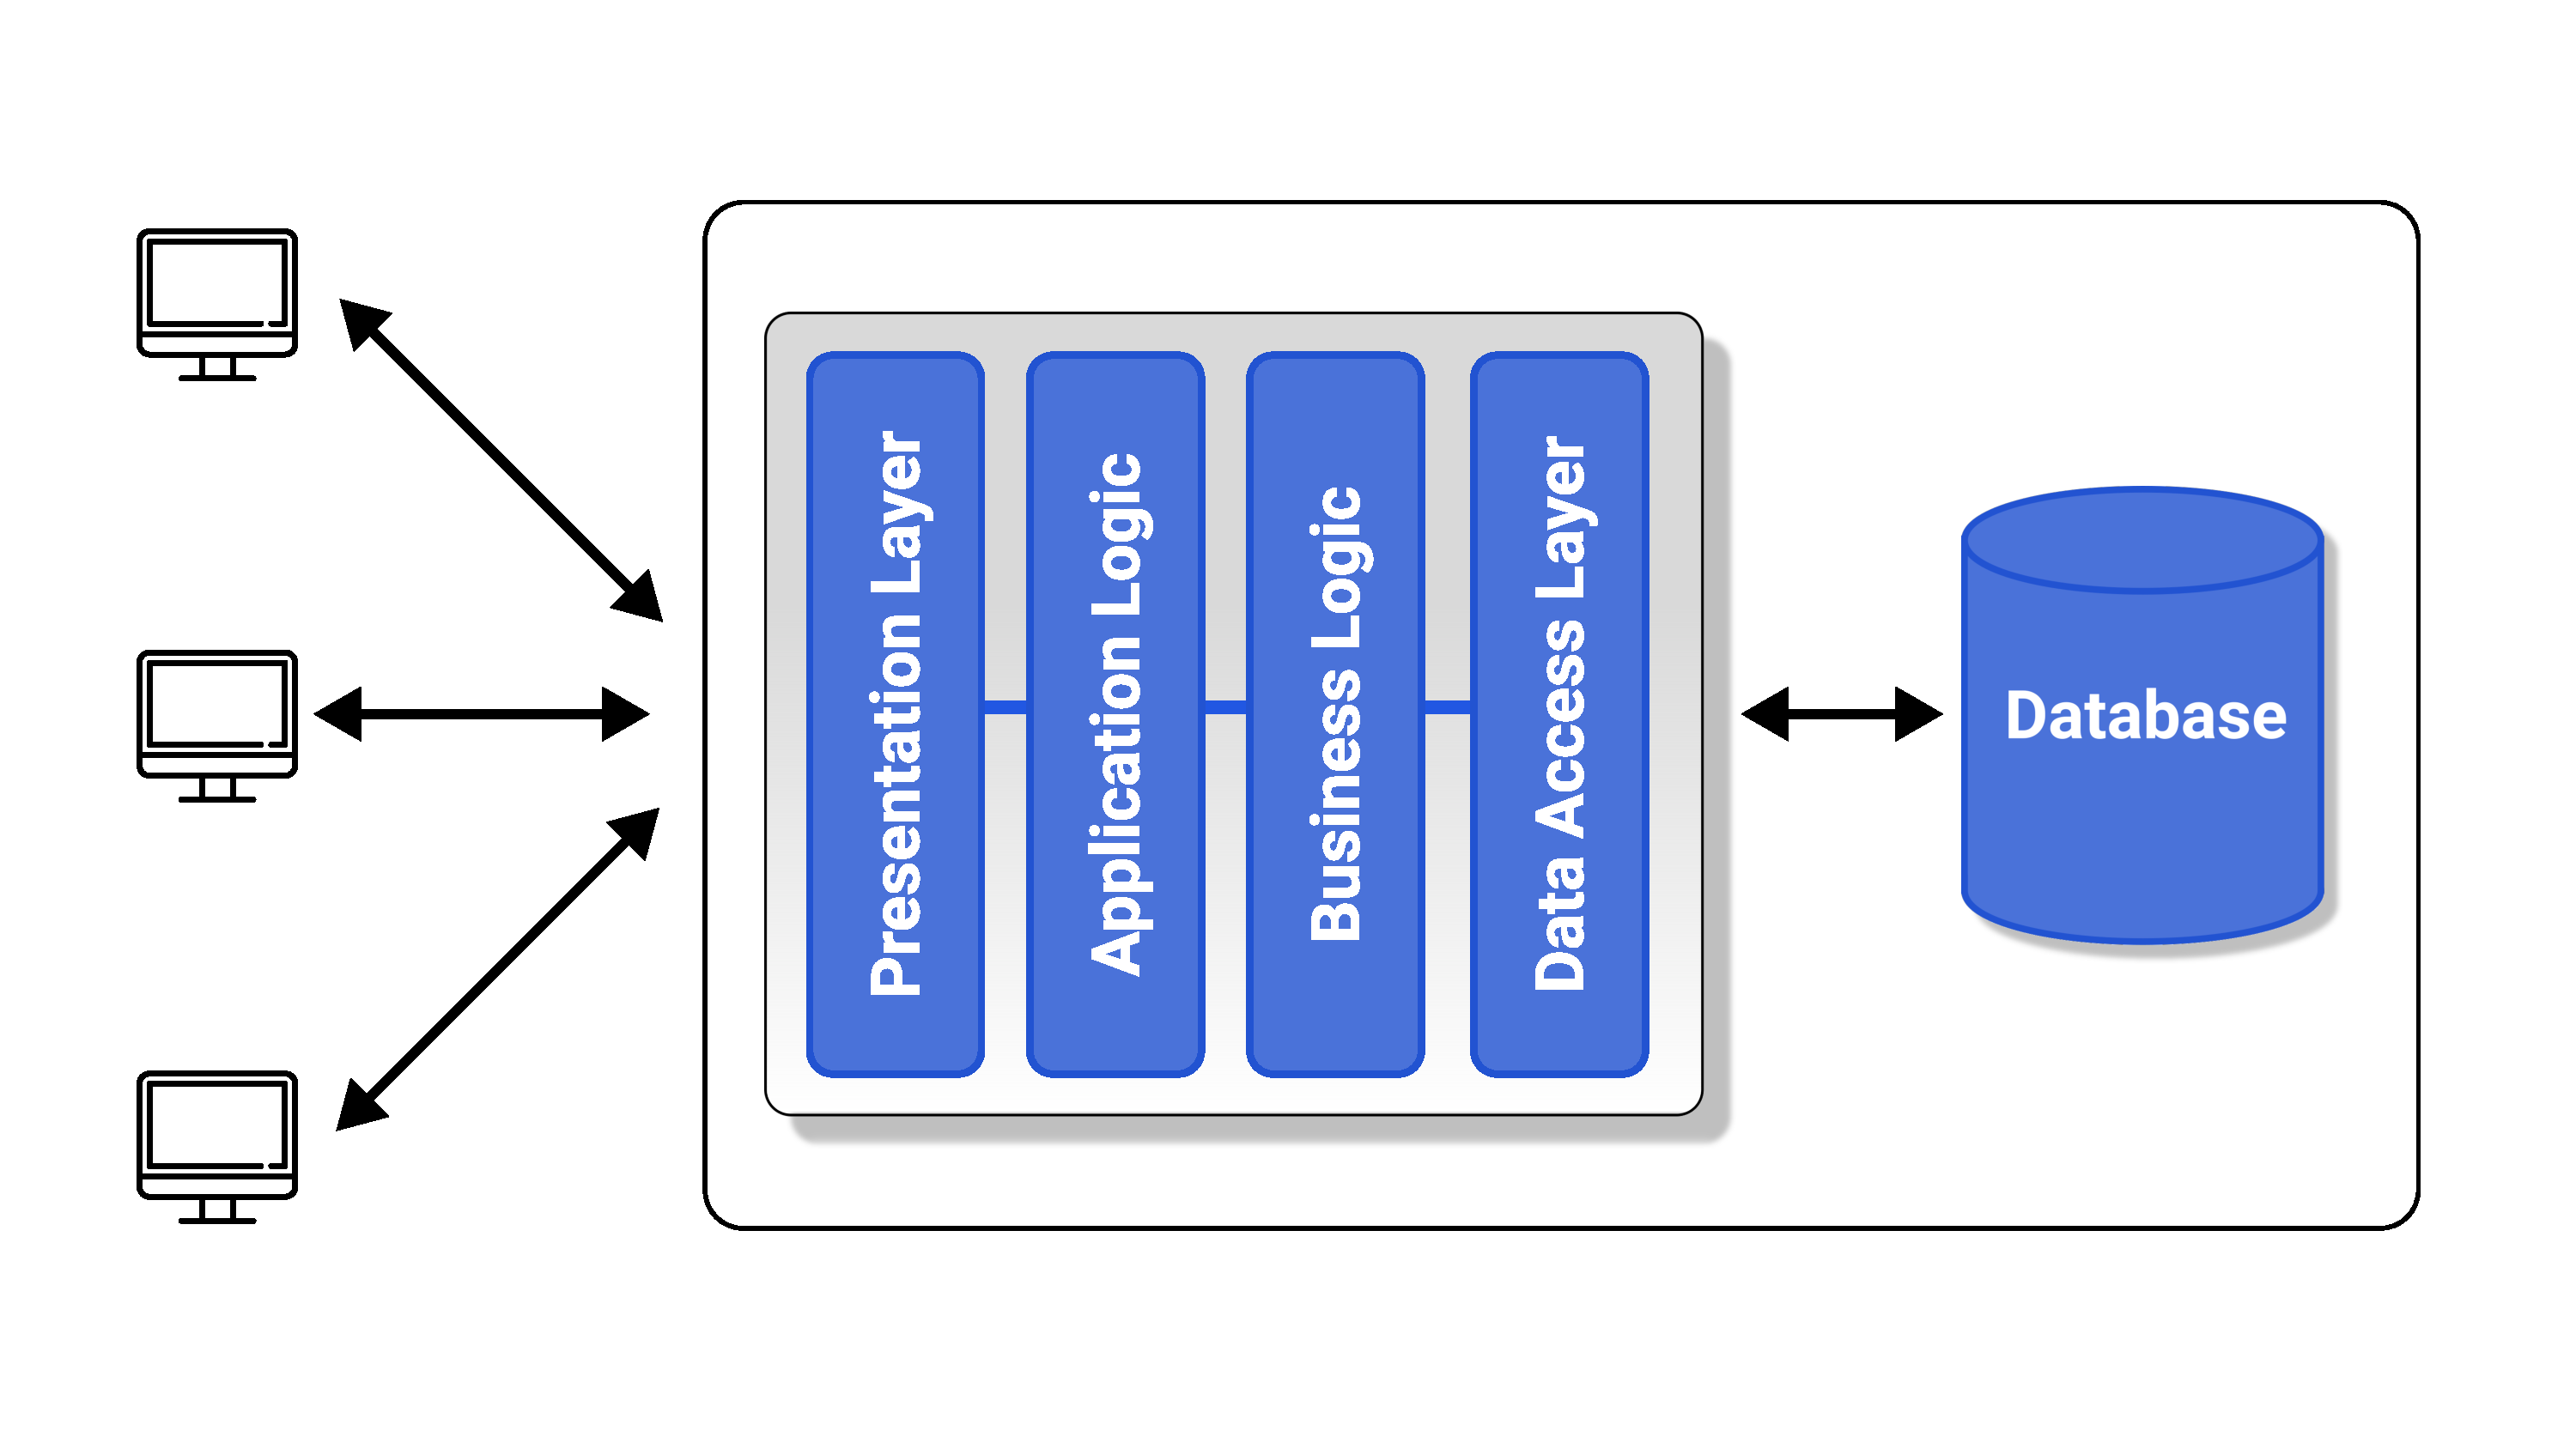
\includegraphics[width=1\textwidth]{Pictures/03_Monolith_concept_diagram}
    \caption{Monolith concept diagram.}\label{fig:figure2}
\end{figure}

\textbf{Monolithic Architecture: Cons and Props.} A monolith is built as a large system with a single code base and
deployed as a single unit, usually behind a load balancer.
Monoliths offer several advantages, particularly when it comes to operational overhead requirements.
Here are some of those basic benefits:

\begin{itemize}
    \item \textit{Simplicity.} Monolithic architectures are simple to build and deploy.
    These applications can scale horizontally, by running several copies of the application behind a load balancer.
    With a single codebase, monolithic apps can easily handle cross-cutting concerns, such as logging,
    configuration management and performance monitoring.
    Another advantage associated with the simplicity of monolithic applications is easier deployment.
    When it comes to monolithic applications, you do not have to handle many deployments but just one.
    \item \textit{Performance.} Components in a monolith typically share memory which is faster than service-to-service
    communications using IPC [\cite{proctor1999linux}] or other mechanisms.
    \item \textit{Easier debugging and testing.}
    In contrast to the microservices, monolithic applications are much easier to debug and test.
    Since that monolithic application is a single indivisible unit the process of end-to-end testing is much faster.
    \item \textit{Easier development.} As long as the monolithic approach is a standard way of building applications,
    any engineering team has the right knowledge and capabilities to develop a monolithic application.
\end{itemize}

However, the drawback of monolithic architectures hides in their tight coupling.
Over time, monolithic components and layers become tightly coupled and entangled, effecting management, scalability
and continuous deployment.
Another disadvantages of the monoliths include:
\begin{itemize}
    \item \textit{Understanding.} When a monolithic application's code base grows up, it becomes too complicated to understand.
    Obviously, huge code base of monolithic app is hard to manage therefore.
    \item \textit{Reliability.} Entire application down may be caused by an error in every single component.
    \item \textit{Updates.} Single and large code base causes the needs to redeploy an application on every single update.
    \item \textit{Technology stack.} Technology stack of the monolithic app is limited by the technologies and providers
    used from the beginning of development.
    It makes technology stack changes to be expensive in terms of finances and time.
    \item \textit{Scalability.} Application's components cannot be scaled independently, an entire application should be scaled.
\end{itemize}

\textbf{Minimization of services coupling.} As we see, the monolith has its own disadvantages, like for instance:
understanding the project structure, reliability concerns, technology stack limitations, scalability limitations.
Obviously, some of these disadvantages cannot be mitigated because of the nature of the monolith.
However, the complexity and coupling problem can be minimized applying certain approaches.
Frequent violation of the single-responsibility principle of SOLID during implementing service components
in business logics layer causes the over-complication of codebase over the time.
The reason is that service components keep the huge number of methods in order to handle all possible CRUD requests
to the database without any bounded context.
Although, the SOLID rules are very powerful in solving designated code issues, it is necessary to apply them very carefully,
since that most of them require high level of abstractions, which increases in size the code base and complicates the
solution.
Do not overcomplicate the solution without any reason following \textit{Open-Closed Principle}.
Schematically, the service entity is as follows
\begin{figure}[H]
    \centering
    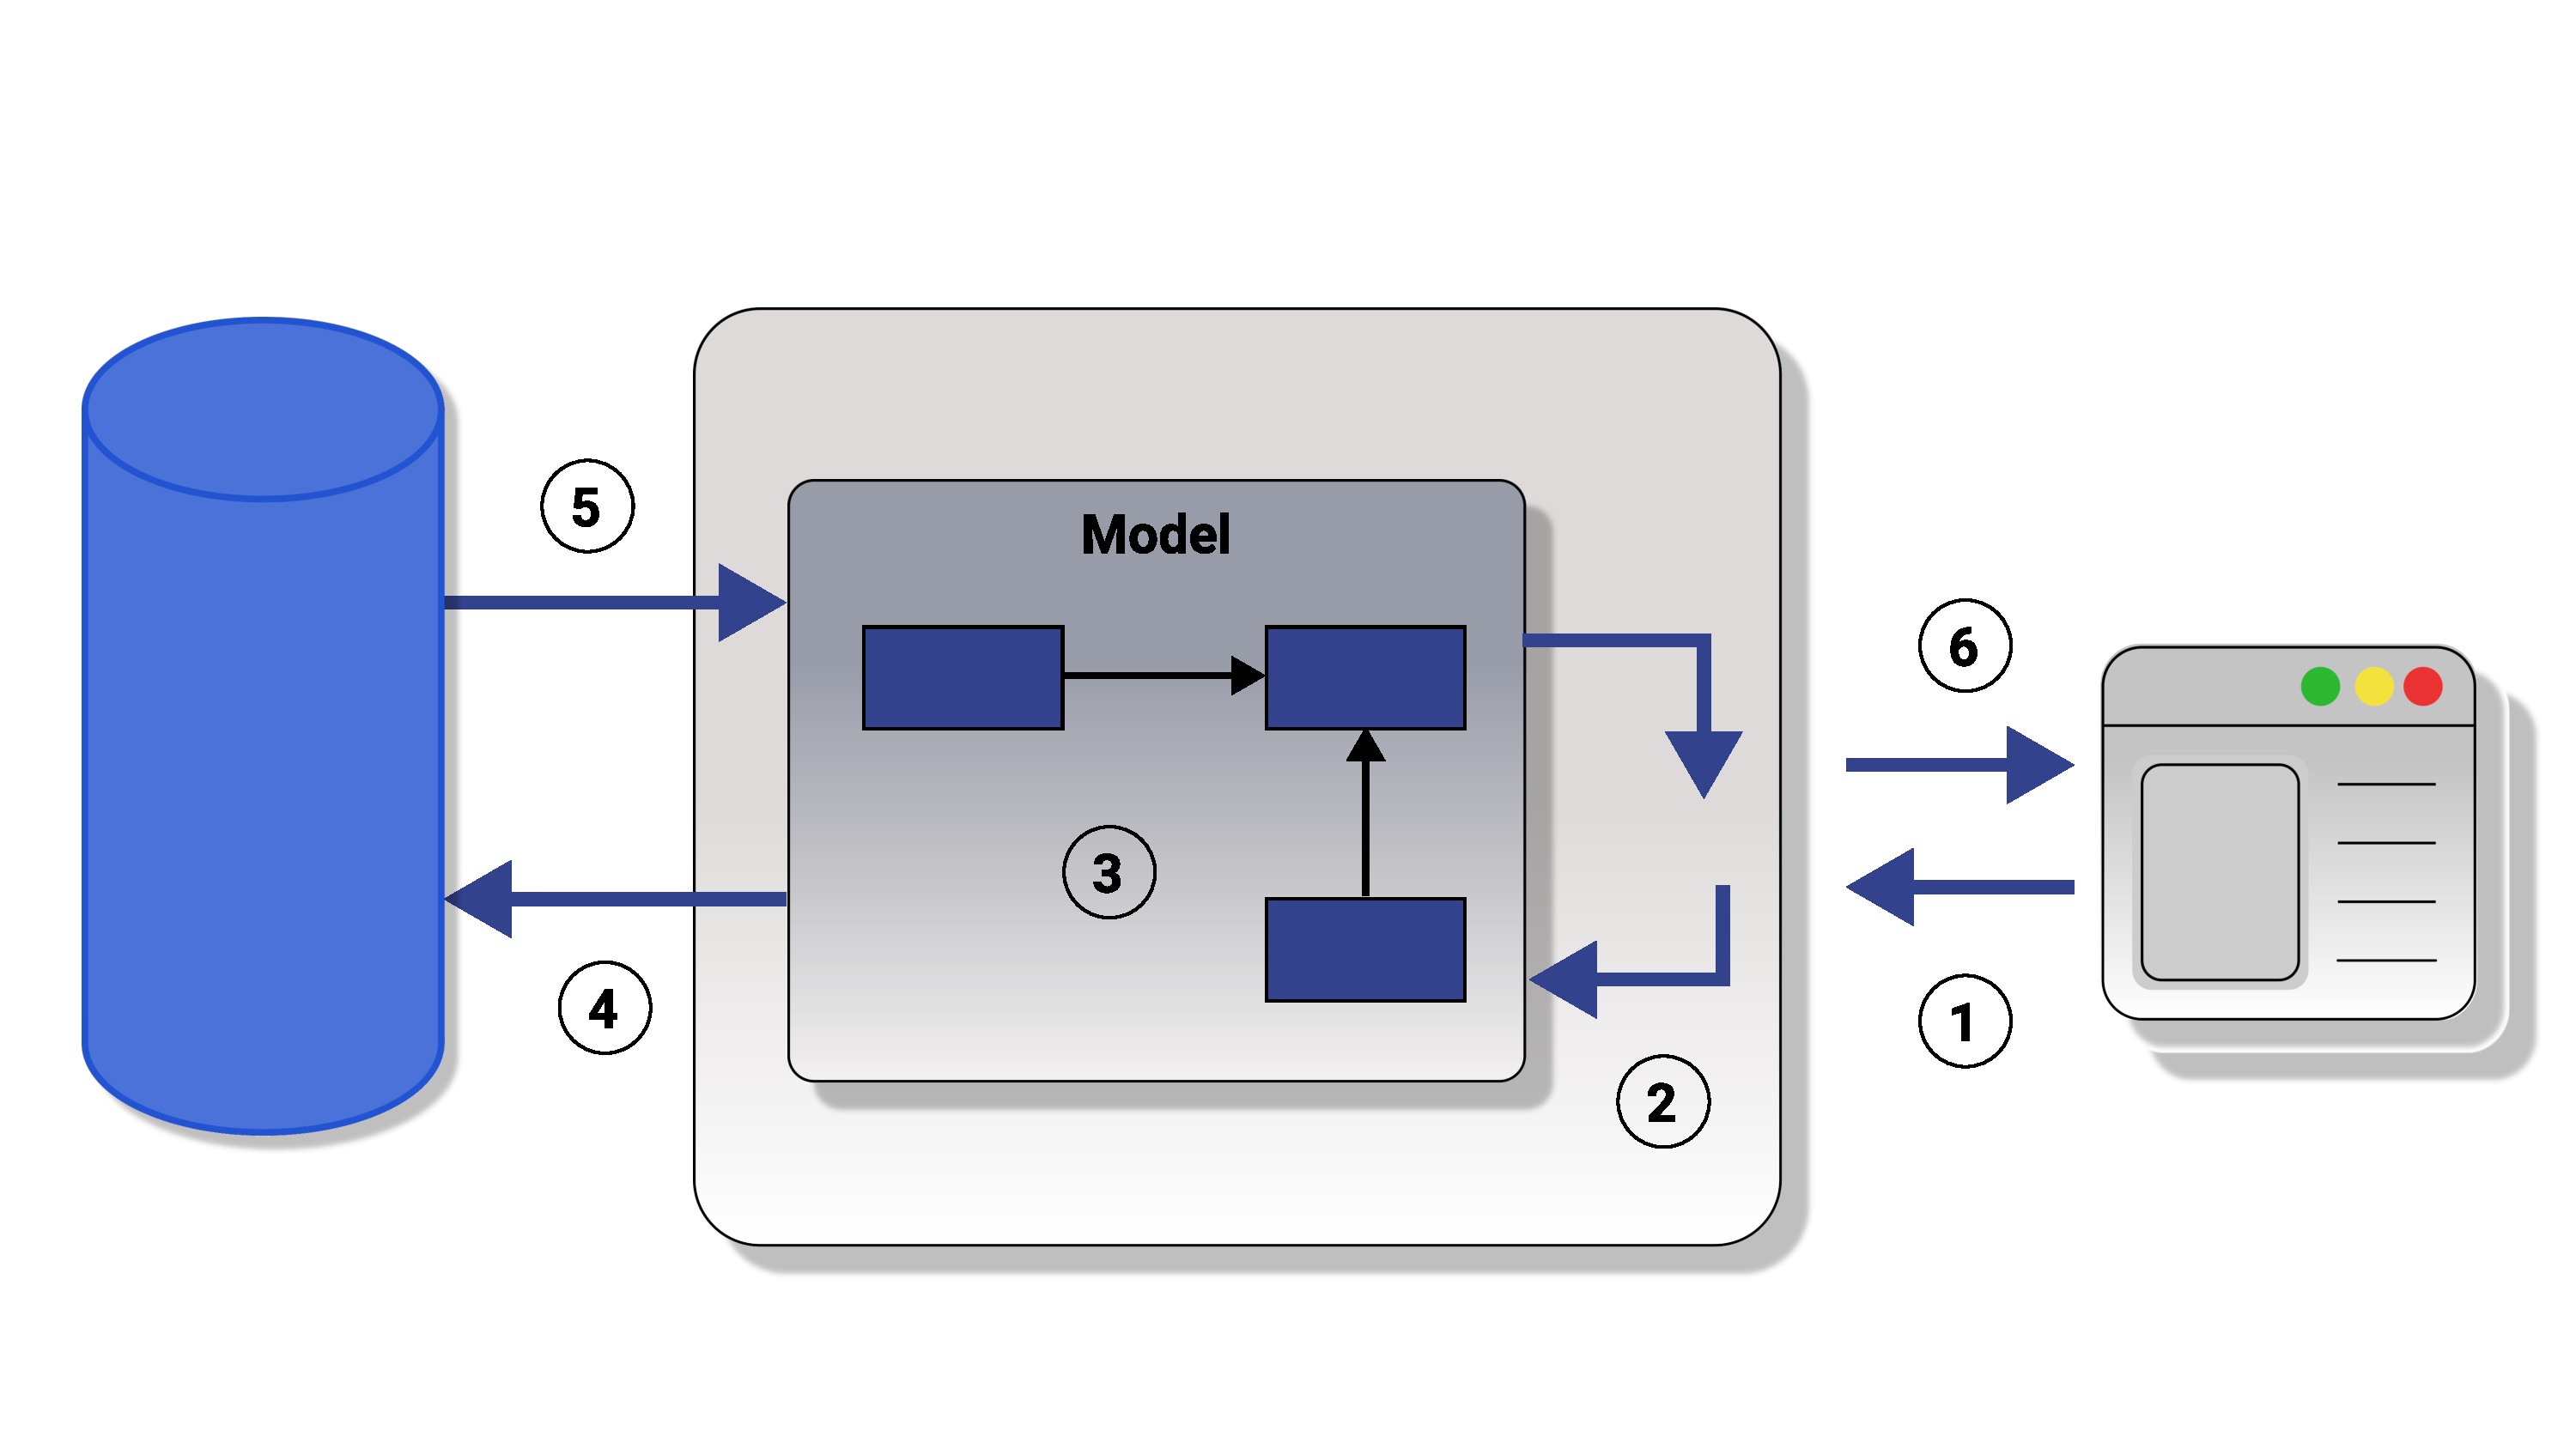
\includegraphics[width=1\textwidth]{Pictures/04_Service_entity_concept_diagram}
    \caption{Service entity concept diagram.
    Source: \href{https://martinfowler.com/bliki/CQRS.html}{Martin Fowler}.}\label{fig:figure9}
\end{figure}
Where the steps are
\begin{enumerate}
    \item User makes a change in UI\@.
    \item Change forwarded to model.
    \item Model executes validation and business logic.
    \item Model updates the database.
    \item Model reads from database.
    \item Service updates presentation from query model.
\end{enumerate}

To minimize the natural disadvantages of the monolithic architecture like complexity and high tight coupling of the components
we have to recall the design patterns [\cite{rising1998design}].
In particular, the mediator pattern helps to decouple the components.
Mediator -- is a behavioral design pattern [\cite{rasche2016building}] that allows the communication between two entities,
such that entities doesn't know each other.
Therefore, the program components depend only on a single mediator instance instead of being coupled to multiple of their
colleagues.
In context of .NET platform there are many implementations of the Mediator, the most widely known and used is the
\href{https://github.com/jbogard/MediatR}{MediatR}, which we use in our project.

Another mindset we are going to use in order to minimize complexity and coupling of monolith is Command-Query
Responsibility Segregation (CQRS) principle.
In brief, it stands that read (query) and write (command) requests should be segregated by their responsibilities.
Using CQRS and Mediator together greatly simplifies the project structure and minimizes coupling between business
logic layer components.
CQRS is a pattern that first described by Greg Young [\cite{young2010cqrs}] and its conceptual diagram as follows

\begin{figure}[H]
    \centering
    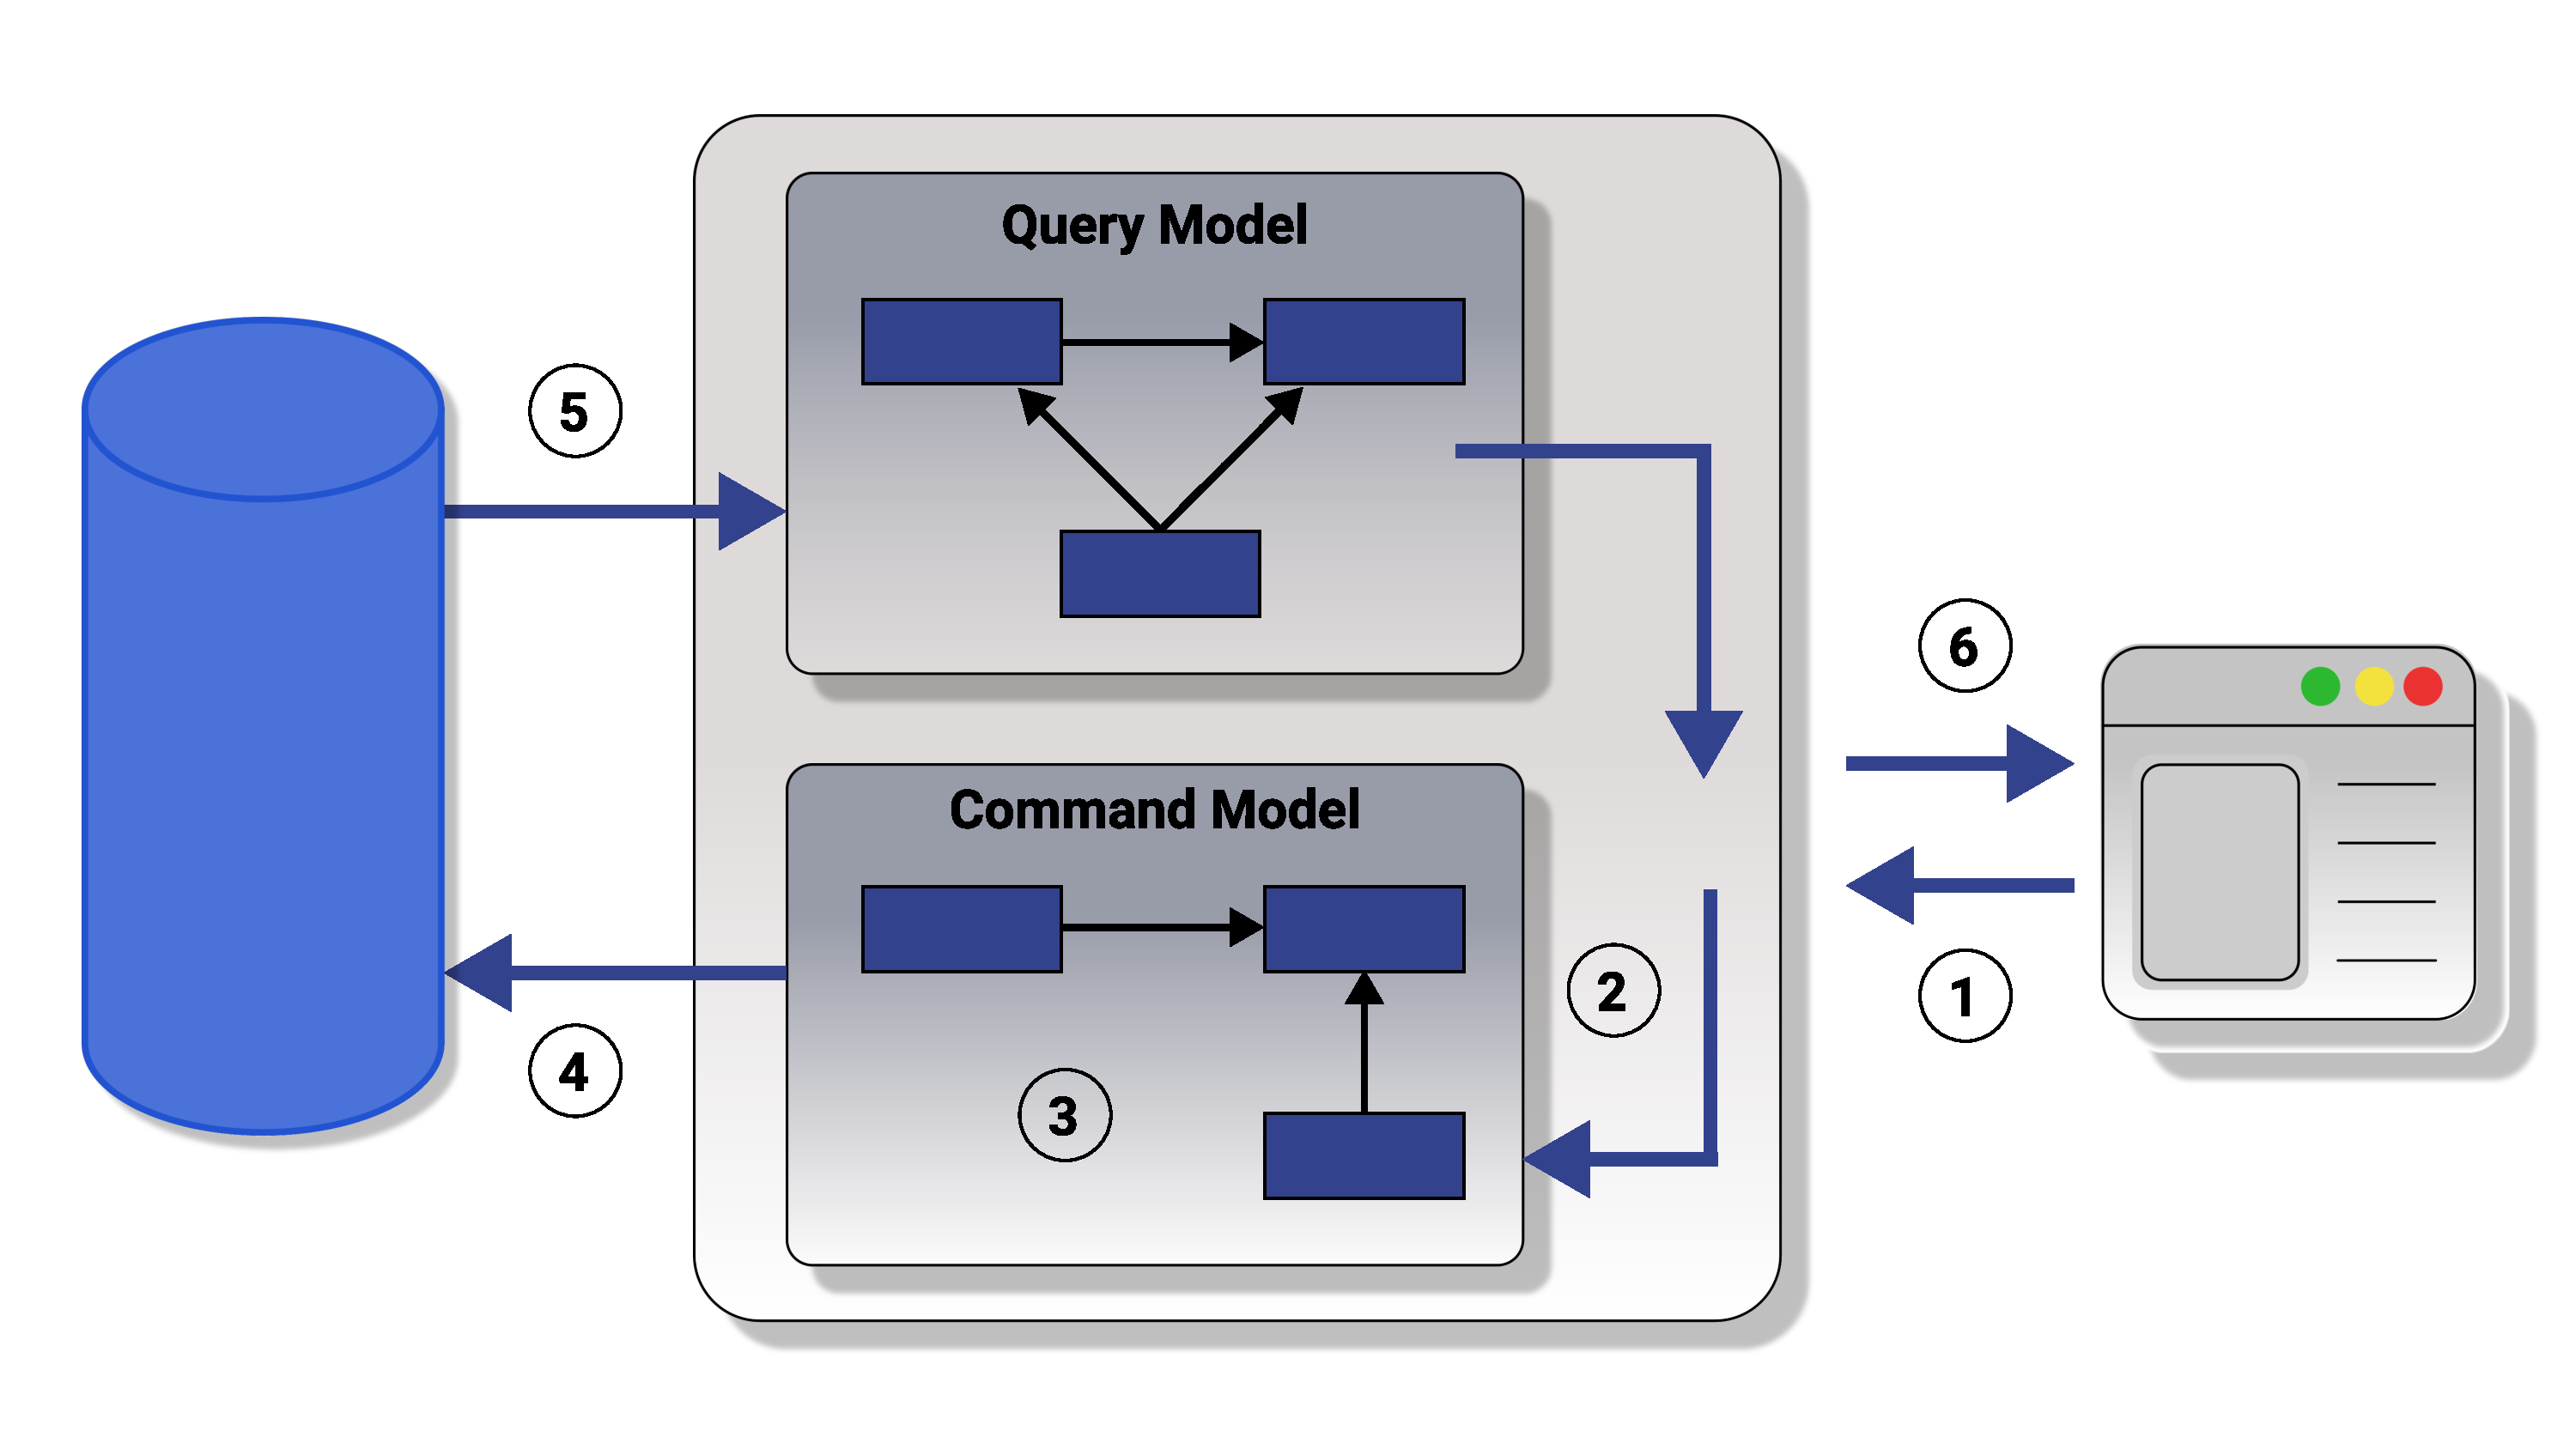
\includegraphics[width=1\textwidth]{Pictures/05_CQRS_concept_diagram}
    \caption{CQRS concept diagram.
    Source: \href{https://martinfowler.com/bliki/CQRS.html}{Martin Fowler}.}
    \label{fig:figure}
\end{figure}

\begin{enumerate}
    \item User makes a change in UI\@.
    \item Application routes information to command model.
    \item Command model executes validation and business logic.
    \item Command model updates the database.
    \item Query model reads from database.
    \item Query service update presentation from query model.
\end{enumerate}